\documentclass[10pt, a4paper]{scrartcl}

\usepackage{vorschule}
\usepackage[
    typ=ab,
    fach=Informatik,
    lerngruppe={EF},
    nummer={I.5},
    module={Symbole,Lizenzen},
    seitenzahlen=keine,
    farbig,
    lizenz=cc-by-nc-sa-4,
]{schule}

\usepackage[
	kuerzel=Ngb,
	reihe={Informationen, Daten und Codierung},
	version={2020-09-7},
]{ngbschule}

\author{J. Neugebauer}
\title{Diagnose Fehlerkorrigierende Codes}
\date{\Heute}

\setzeAufgabentemplate{ngbnormal}

\usetikzlibrary{matrix}

\tikzstyle{card deck}=[scale=1,every node/.style={transform shape}]
\tikzstyle{card}=[draw,fill=gray!10,rectangle,minimum width=10mm,minimum height=10mm,anchor=south west]
\tikzstyle{white card}=[card,fill=white]
\tikzstyle{black card}=[card,fill=black]
\tikzstyle{card bg}=[draw=black,fill=black!30]

\begin{document}

\ReiheTitel

\begin{aufgabe}
Markiere in der ersten Reihe und letzten Spalte die Karten, die nach dem Prüfbit-Verfahren \enquote{schwarz} sein müssen.
\begin{multicols}{2}
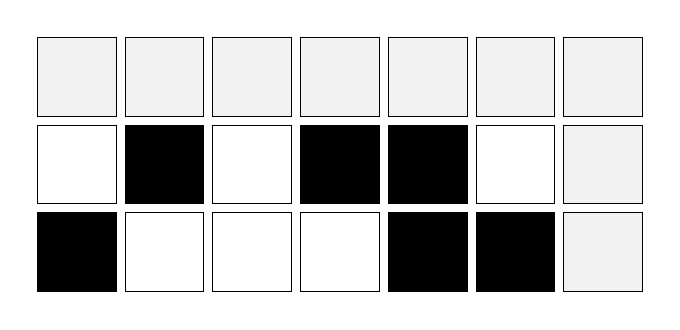
\begin{tikzpicture}
\matrix (m) [matrix of nodes,column sep=1mm,row sep=1mm,anchor=center] {
	|[card]| & |[card]| & |[card]| & |[card]| & |[card]| & |[card]| & |[card]| \\
	|[white card]| & |[black card]| & |[white card]| & |[black card]| & |[black card]| & |[white card]| & |[card]| \\
	|[black card]| & |[white card]| & |[white card]| & |[white card]| & |[black card]| & |[black card]| & |[card]| \\
};
\end{tikzpicture}

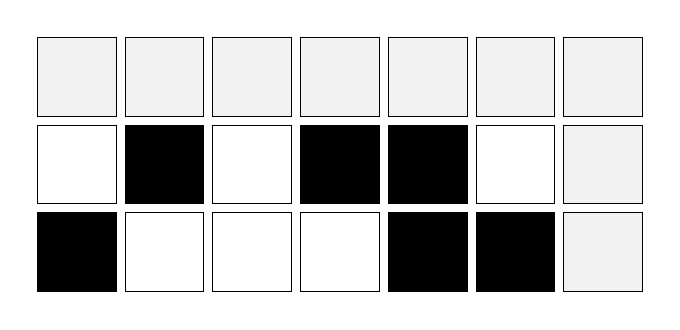
\begin{tikzpicture}
\matrix (m) [matrix of nodes,column sep=1mm,row sep=1mm,anchor=center] {
	|[card]| & |[card]| & |[card]| & |[card]| & |[card]| & |[card]| & |[card]| \\
	|[white card]| & |[black card]| & |[white card]| & |[black card]| & |[black card]| & |[white card]| & |[card]| \\
	|[black card]| & |[white card]| & |[white card]| & |[white card]| & |[black card]| & |[black card]| & |[card]| \\
};
\end{tikzpicture}
\end{multicols}
\end{aufgabe}

\end{document}